\documentclass[../main.tex]{subfiles}

\begin{document}

\section{Pavimentos flexibles}

Normalmente se pueden utilizar los métodos Porter o método Shell. El más
preferido es el último, que permitió el avance de muchas cosas en cuanto a 
como se realizaban.

\subsection{Método Shell}

Este método asume que se encuentra una estructura bien diseñada, que se comporta
elásticamente bajo acción de las cargas dinámicas. 

\begin{figure}[htpb]
  \centering
  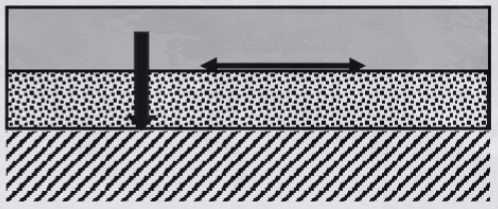
\includegraphics[width=0.8\textwidth]{../images/20210527/shell}
  \caption{Esfuerzos críticos}
  \label{fig:shell}
\end{figure}

Se deben considerar los siguientes \textbf{esfuerzos críticos}:

\begin{description}
  \item[Excesiva deformación de la superficie] por acumulación de pequeñas 
    deformaciones permanentes en la estructura. En estructuras bien diseñadas,
    estas son primariamente dependientes de la compresión vertical en la 
    superficie de la subrasante.
  \item[Rotura de la capa asfáltica] por la flexión repetida de esta capa bajo
    las cargas del tráfico. El inicio de tales roturas es gobernada por la 
    tracción en el borde inferior de la capa asfáltica.
\end{description}

\subsubsection{Parámetros de diseño}

Para la \textbf{subrasante} se considera el VSR o Valor Soporte Relativo, y en
el \textbf{tránsito}, se considera un número \textit{N}, que es la cantidad total
de ejes equivalentes a $\SI{10}{tn}$ que pasan por la trocha más cargada durante
la vida útil. Es equivalente a:

\begin{align*}
  N_{10t} = N_x*\left(  \frac{x}{10}\right)^4
.\end{align*}

\subsubsection{Cartas de diseño}

En X se da el espesor de la capa granular total, y en Y se da el espesor de la 
capa asfáltica. En la misma se encuentran dos curvas, que dan las cargas 
críticas que corresponden a un \textit{N} en particular. Esto se ve en \Cref{fig:carta_shell}

\begin{figure}[htpb]
  \centering
  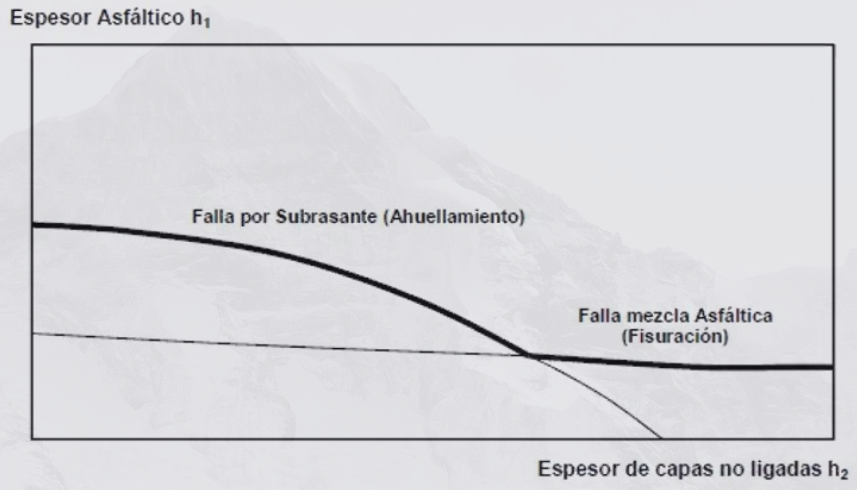
\includegraphics[width=0.8\textwidth]{../images/20210527/carta_shell}
  \caption{Carta Shell VSR}
  \label{fig:carta_shell}
\end{figure}  

Lo que se busca que el punto se encuentre sobre las curvas mostradas, ya que
menos no serán suficientes, y sobre la misma se estaría sobre dimensionando.



\end{document}                                                           
                                                                         
                                                                          
